\documentclass[a4paper]{article}
\usepackage[left=1.5cm,right=1.5cm]{geometry}
\usepackage{ctex}
\usepackage{graphicx}
\usepackage{siunitx}
\usepackage{float}
\usepackage{hyperref}
\usepackage{enumerate}
\usepackage[thehwcnt = 3]{iidef}
\thecourseinstitute{清华大学}
\thecoursename{计算机网络原理}
\theterm{2023年秋季学期}
\hwname{作业}
\begin{document}
\courseheader
\name{杨哲涵}
\section{第三章习题}
\paragraph{1}
不加处理的情况下会造成帧被错误地分割.因此通常的做法是用转义字符替代前导码.
\paragraph{2}
\verb|A B ESC ESC C ESC ESC ESC FLAG ESC FLAG D|
\paragraph{4}
\verb|0110 0111 1101 1110 11111 1|
\paragraph{5}
不是很理解这道题的意思,如果指的是Internet checksum.那么单个比特的错误有可能不被检测出来.例如:

\verb|0001|错误插入了一个\verb|0|比特,变成\verb|000010|.假设校验和计算方法为从头开始每4位作为一个整数采用一补数相加,那么最后加0不改变结果.这个错误没有被检测到.
\paragraph{6}
一次发送成功的概率为$0.8^{10}$.平均需要发送$1/0.8^{10}=9.31$次.
\paragraph{11}
数据为\verb|10101111|,偶校验海明编码后为\verb|hh1h010h1111|.可以参考\url{https://www.wikiwand.com/zh/Hamming_code}进行计算,结果为\verb|101001001111|
\paragraph{13}
收到\verb|101101001101|,可以发现没有错误.
\paragraph{24}
首先补齐3个\verb|0|,得到\verb|10011101000|,接着长除\verb|1001|,得到商为\verb|100|.结果为\verb|10011101000-100=10011101100|.
\paragraph{28}
设帧长为$l$,有$\frac{l/4}{l/4+20+20}>0.5$,可得$l>320$.因此需要帧长超过320比特.
\paragraph{29}
B的效率应当为A的20分之一,即5\%.
\paragraph{33}
对于旧信道的$BD$,我们知道$2BD+1=3$,有$BD=1$.升级为新信道后,$BD$变为2,$w$变为5,如果维持原先的协议不变,带宽效率为$2/5=60\%$.
\paragraph{35}
可算得$BD=54.28125$,有$w=109.5625<2^7$,取序号长度为7位比较合理.
\paragraph{42}
每次发送后会触发一次超时重传,平均传输2次.
\paragraph{44}这种情况下$BD=270$,$w=2BD+1=541$.
a. 信道利用率为1/541=0.185\%.

b. 利用率为8/541=1.48\%.

c. 利用率为8/541=0.739\%.
\section{PPPoE实验}
\begin{figure}[H]
    \centering
    \begin{minipage}[t]{0.45\linewidth}
        \centering
        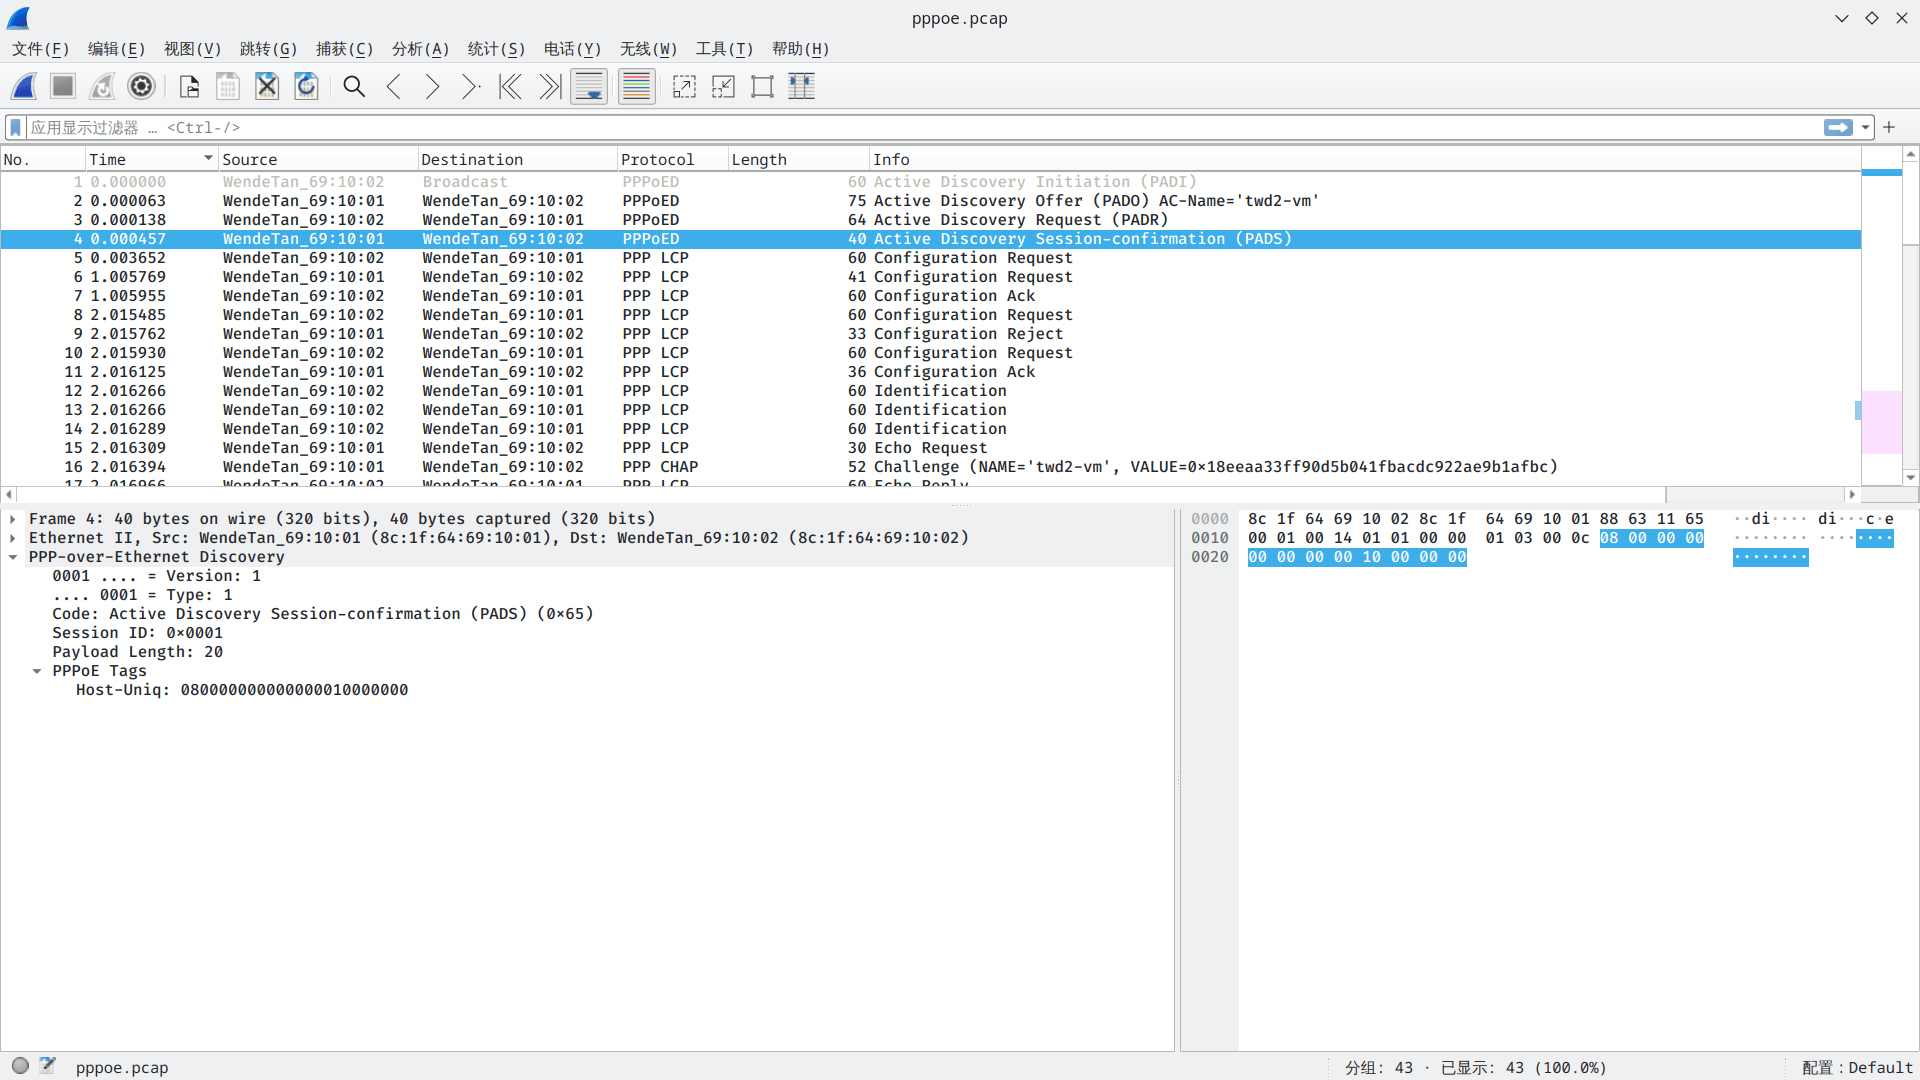
\includegraphics[width=\linewidth]{PPPoE-1.png}
        \caption{PADS}
        \label{1}
    \end{minipage}
    \begin{minipage}[t]{0.45\linewidth}
        \centering
        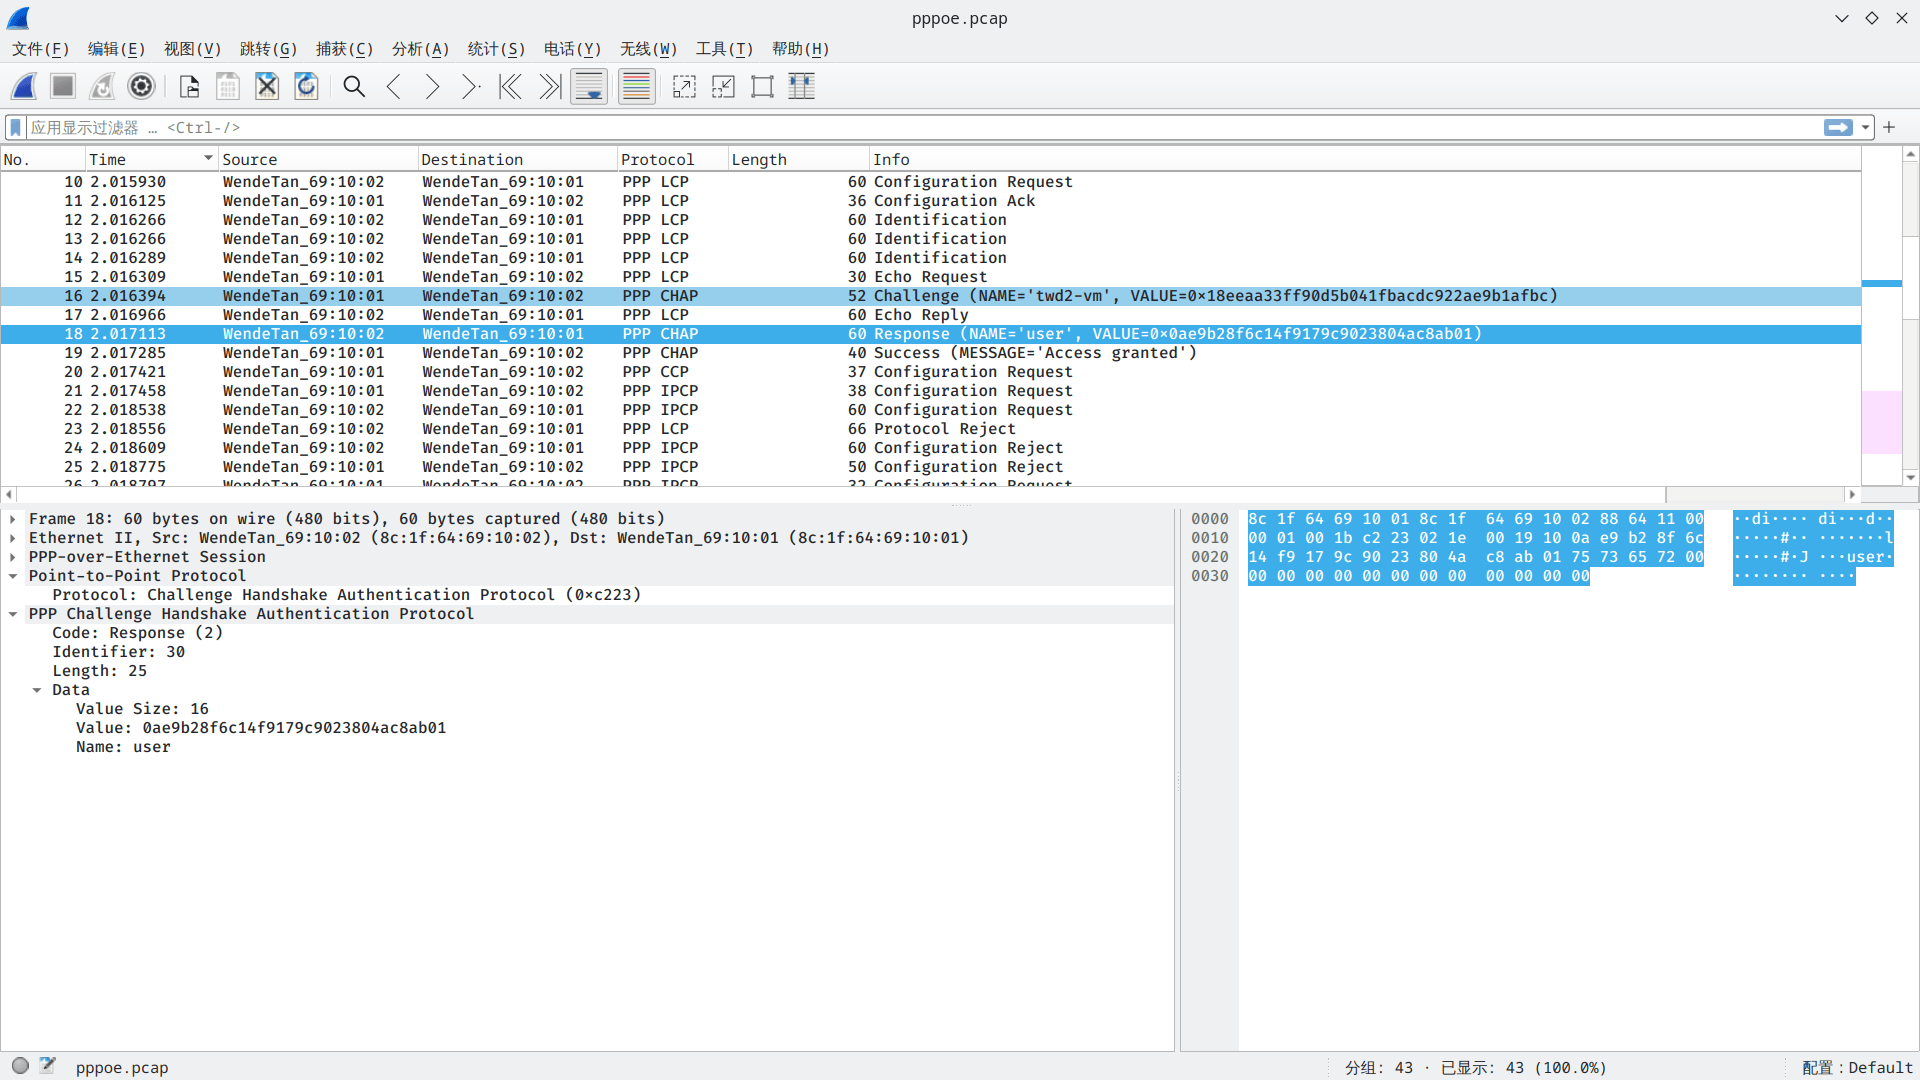
\includegraphics[width=\linewidth]{PPPoE-2.png}
        \caption{PPP CHAP Response}
        \label{2}
    \end{minipage}
    \begin{minipage}[t]{0.45\linewidth}
        \centering
        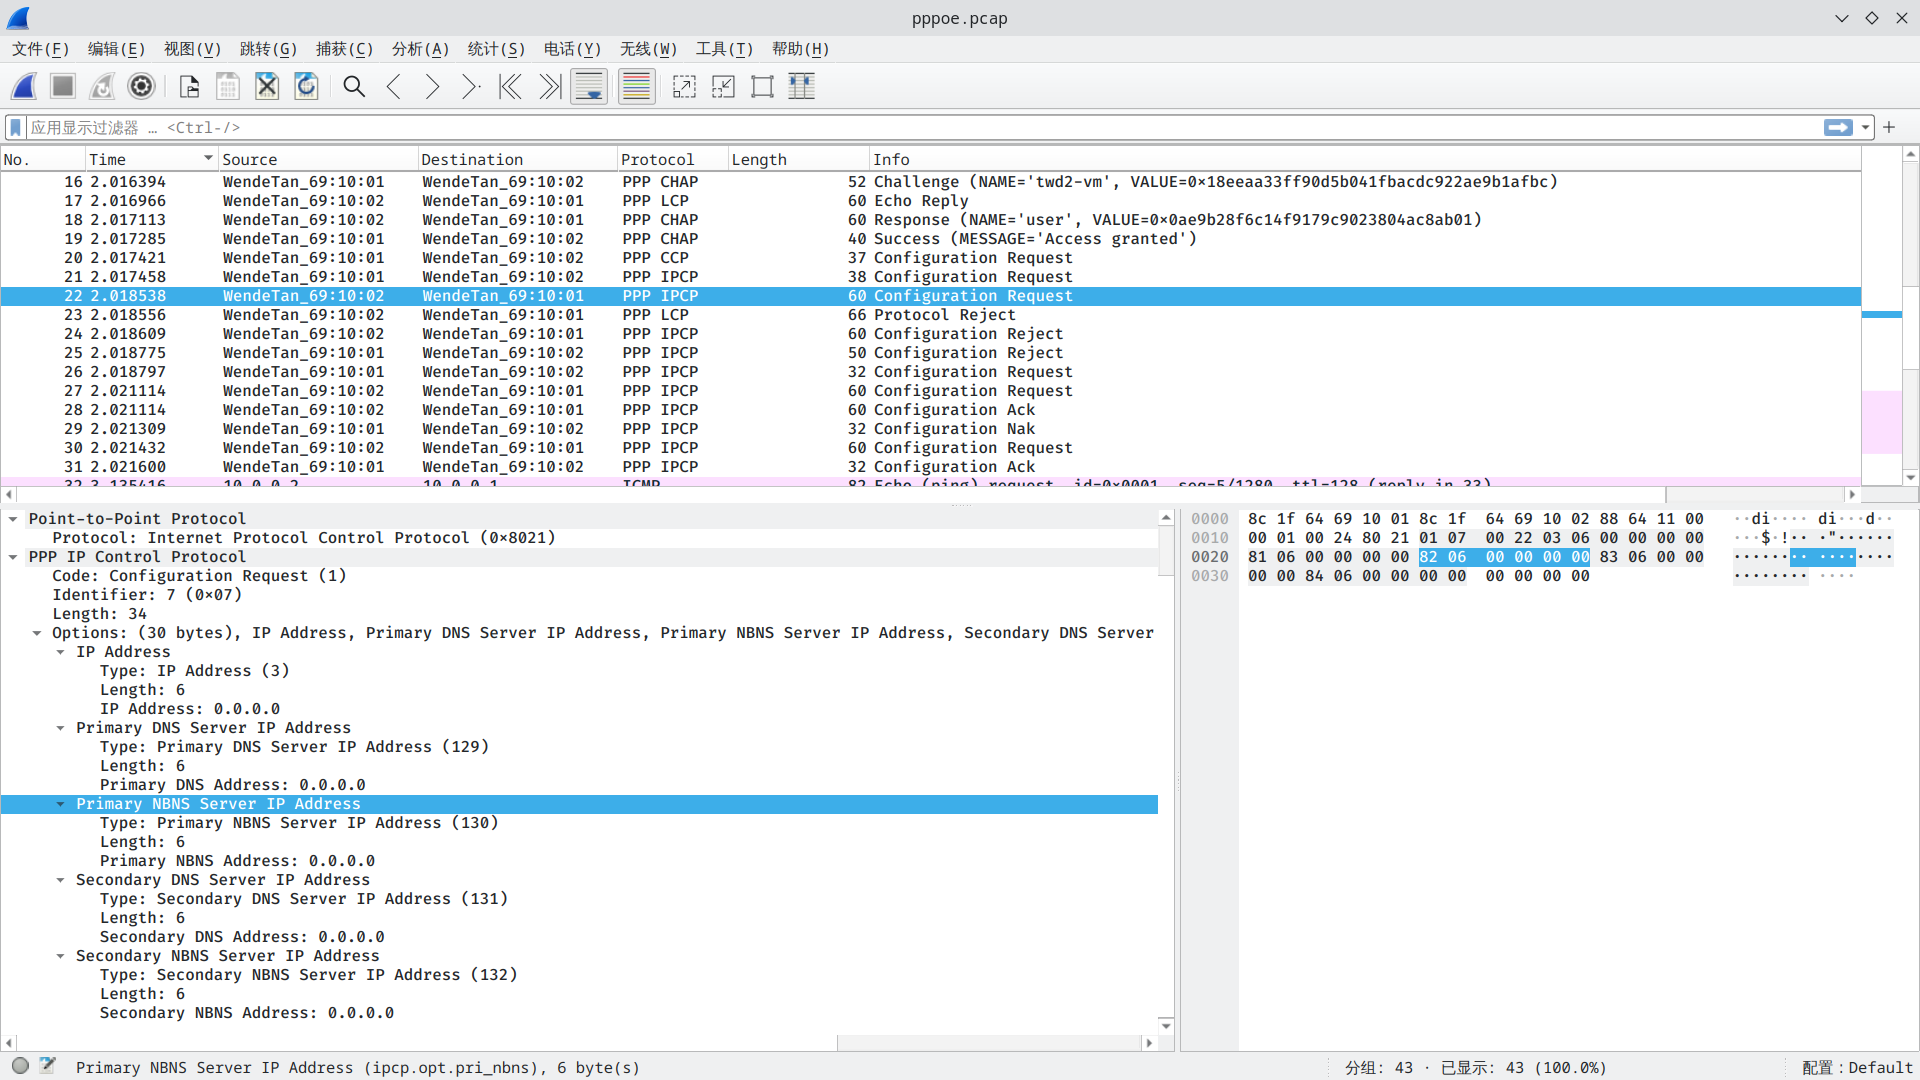
\includegraphics[width=\linewidth]{PPPoE-3.png}
        \caption{PPP IPCP Request}
        \label{3}
    \end{minipage}
    \begin{minipage}[t]{0.45\linewidth}
        \centering
        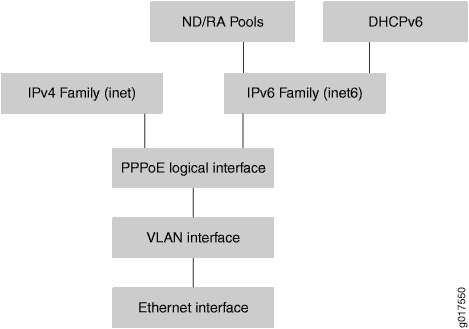
\includegraphics[width=\linewidth]{PPPoE-4.png}
        \caption{PPPoE双栈接入}
        \label{4}
    \end{minipage}
\end{figure}
PADS报文见图\ref{1}.PPPoE服务器的地址是\verb|8c1f64691001|,PPPoE客户端的地址是\verb|8c1f64691002|
\paragraph{2}
PPP CHAP Response与PPP IPCP Request报文见图\ref{2},\ref{3}.

PPP CHAP Response的加密摘要字段为\verb|0ae9b28f6c14f9179c9023804ac8ab01|.
\paragraph{3}
认为MTU即以太网DMAC,SMAC,Type后容纳的数据最多为1500字节.考虑PPPoE协议占用6个字节,PPP协议(PPPoE封装)占用2个字节,IPv4占用20个字节,UDP占用8个字节,那么上层应用能使用的最大容量为1464个字节.
\paragraph{4}
这是为了避免浪费字节.因为PPPoE中已经有VER,TYPE,CODE,SESSIONID字段.所以不必在PPP协议头中重复.
\paragraph{5}
MRU一般为1492字节,这是因为以太网MTU=1500字节,减去PPoE,PPP后为1492.此外MRU受到协商接受能力的限制.
\paragraph{6}
根据\url{https://www.juniper.net/documentation/cn/zh/software/junos/subscriber-mgmt-sessions/topics/topic-map/dual-stack-pppoe-access-monitoring-and-management.html},一种方案是IPv4与IPv6双栈共用PPPoE的逻辑接口,通过DHCPv6服务器解决IP地址分配的问题(参见图\ref{4}).这是一种兼容性很好的方案.
\paragraph{7}
PPPoE的优点是提供了一种身份验证方案,方便ISP提供商的计费,这种拨号上网方式非常流行.但是缺点在于需要额外的PPPoE服务器来管理,有额外冗余.现在有IPoE等技术,也有其他的不依赖PPPoE的准入管理方案(例如校园网).
\end{document}
